%%%%%%%%%%%%%%%%%%%%%%%%%%%%%%%%%%%%%%%%%%%%%%%%%%%%%%%%%%%%%%%%%%%%%%%%%%%%%%%%
% \documentclass[12pt,papel,twoside]{ibtesis}
% \documentclass[12pt,papel,singlespace,oneside]{ibtesis}
% \documentclass[12pt,papel,preprint,singlespace,oneside]{ibtesis}

\documentclass[screen,pagebackref]{ibtesis}
% Antes acá estaba
% \documentclass[12pt,screen,twoside,pagebackref]{ibtesis}


%%%%%%%%%%%%%%%%%%%%% Paquetes extra %%%%%%%%%%%%%%%%%%%%%%%%%%%%%%%%%%%%%%%%%%%
% Por conveniencia: aqu\'{\i} puede cargar todos los paquetes y definir los comandos 
% que necesite
\usepackage{ibextra}
\usepackage{subcaption}


\usepackage{todonotes}
\usepackage{pdfcomment}
\usepackage{listings}
\usepackage{xcolor}  % for coloring
\renewcommand{\lstlistingname}{Código}
\renewcommand{\lstlistlistingname}{Índice de códigos}

\lstset{
  language=C,                   % Idioma del código
  basicstyle=\ttfamily\small,  % Fuente monoespaciada pequeña
  keywordstyle=\color{blue}\bfseries, % Palabras clave en azul y negrita
  commentstyle=\color{gray},   % Comentarios en gris
  stringstyle=\color{red},     % Cadenas en rojo
  numbers=left,                % Numerar líneas a la izquierda
  numberstyle=\tiny,           % Tamaño de los números de línea
  numbersep=5pt,               % Separación de los números
  backgroundcolor=\color{white}, % Fondo blanco
  frame=single,                % Marco alrededor del código
  breaklines=true,             % Romper líneas largas
  captionpos=b,                % Colocar el título debajo del código
  literate={á}{{\'a}}1 {é}{{\'e}}1 {í}{{\'i}}1 {ó}{{\'o}}1 {ú}{{\'u}}1 {ñ}{{\~n}}1 {Ñ}{{\~N}}1, % Soporte para caracteres especiales
  extendedchars=true,
  inputencoding=utf8
}


%\usepackage{hyphen-spanis}
%%%%%%%%%%%%%%%%%%%%%%%%%%%%%%%%%%%%%%%%%%%%%%%%%%%%%%%%%%%%%%%%%%%%%%%%%%%%%%%%
%%%%%%%%%%%%%%%%%%%%% Informacion sobre la tesis %%%%%%%%%%%%%%%%%%%%%%%%%%%%%%%
\title{Mi súper interesante PI}
\author{Juan Teleco}
\director{Ing. Pepe Antenil}
%\codirector{Dr.~J.~Otro m\'{a}s}
\carrera{Proyecto Integrador de la Carrera de Ingeniería en Telecomunicaciones}
\grado{Estudiante}
\laboratorio{Telecolandia}
\jurado{Señor Malo 1 (INVAP) \\ 
Señora Mala 2 (Instituto Balseiro)}
\palabrasclave{formato de Tesis, Lineamientos de escritura, Instituto Balseiro}
\keywords{Thesis format, Templates, Instituto Balseiro}
% Si queremos poner la fecha manualmente:
% \date{Diciembre de 2099}

%%%%%%%%%%%%%%%%%%%%%%%%%%%%%%%%%%%%%%%%%%%%%%%%%%%%%%%%%%%%%%%%%%%%%%%%%%%%%%%%
%\titlepagefalse % Si no quiere compilar la portada descomente esta linea
%\includeonly{apendices} % Compilar s\'{o}lo estos archivos 
\graphicspath{{figs/}} % Lugar donde encontrar las figuras generales (se puede poner uno en cada cap{\'{\i}}tulo)
%%%%%%%%%%%%%%%%%%%%%%%%%%%%%%%%%%%%%%%%%%%%%%%%%%%%%%%%%%%%%%%%%%%%%%%%%%%%%%%%


\begin{document}

% Dentro del environment 'preliminary' va:
% la dedicatoria, resumen, abstract, indices

\begin{preliminary}

% Escriba su dedicatoria
\dedicatoria{
A todos los telequitos
}

%%% \'{I}ndices %%%%

\begin{abreviaturas}
                                %Abreviaturas
\end{abreviaturas}

\tableofcontents                %\'{I}ndice

\listoffigures                  %Figuras

\listoftables                   %Tablas

\begin{resumen}%
Este es el resumen en castellano.\\
La tesis debe reflejar el trabajo desarrollado, mostrando la metodolog\'{\i}a utilizada, los resultados obtenidos y las conclusiones que pueden inferirse de dichos resultados.
\end{resumen}

\begin{abstract}%
This is the title in English:\\
The thesis must reflect the work of the student, including the chosen methodology, the results and the conclusions that those results allow us to draw.
\end{abstract}

\end{preliminary}

%% acá deberían incluirse los capítulos
\chapter{Introducción}
\section{Motivación y objetivos}
En el ámbito de las comunicaciones, es fundamental contar con un sistema capaz de garantizar confiabilidad respecto a la autenticación, confidencialidad e integridad de la información transmitida. Cuando la comunicación se desarrolla sobre un medio considerado inseguro, asegurar el cumplimiento de estas propiedades implica abordar desafíos, como mitigar la posibilidad de suplantación de identidad, encriptar la información para asegurar confidencialidad y detectar modificaciones del mensaje por agentes externos.

Se han desarrollado soluciones privativas al problema descrito. Sin embargo, la inexistencia de \textit{back-doors} y mecanismos de vigilancia es algo que no puede ser verificado por completo en dichas soluciones. Es por esto que en áreas como defensa y servicio diplomático es de interés contar con equipos completamente auditables, que no dependan de licencias de exportación. A su vez, que la funcionalidad y validación formal del equipo no dependa de las funciones criptográficas utilizadas, y que estas puedan ser provistas o implementadas por el usuario final.

El continuo aumento del poder de cómputo ha permitido la ejecución de múltiples sistemas operativos sobre un mismo \textit{hardware}. Esto habilitó la adopción de tecnologías de virtualización en sistemas embebidos y de misión crítica. Una de las principales motivaciones detrás de esta tendencia es la capacidad de establecer fronteras fuertes entre dominios con distintos niveles de confianza, como es el caso de los dominios rojo/negro en sistemas de comunicaciones.

En este trabajo se propone un abordaje novedoso a las soluciones de encriptación de redes: la utilización de tecnologías de virtualización para la segmentación de dominios rojo/negro en un encriptador. Los objetivos que se pretenden alcanzar se resumen en los siguientes:
\begin{itemize}
    \item Validar la viabilidad de realizar segmentación virtual de dominios.
    \item Realizar una prueba de concepto del enfoque propuesto.
    \item Implementar una propuesta de solución auditable y documentada.
\end{itemize}

La continuación de este capítulo tiene como propósitos: (i) brindar una visión general sobre conceptos relacionados a sistemas de comunicaciones seguras, (ii) presentar el sistema propuesto y su justificación y (iii) describir los requerimientos para con el sistema a desarrollar.

\clearpage

\section{Concepto de operaciones}
El CONOPS es un documento utilizado para describir cómo se espera que opere un sistema desde el punto de vista del usuario final, sin brindar aún detalles técnicos de la solución. Esta sección es de utilidad para clarificar el propósito y uso del sistema, y  sirve además de base para la definición de requerimientos.

\subsection{Contexto}

La tríada de la CIA \textit{(Confidentiality, Integrity, Availability)} es un modelo que constituye la base para el desarrollo de sistemas de seguridad. Es utilizada para identificar vulnerabilidades de un sistema y proponer soluciones que cumplan con estos principios. 
\begin{itemize}
    \item \textbf{Confidencialidad}: consiste en proteger la información sensible de accesos no autorizados. Los métodos para reforzar este aspecto pueden involucrar la encriptación de la información y la implementación de controles de acceso.
    \item \textbf{Integridad}: refiere a asegurar la consistencia y confiabilidad de la información transmitida y mitigar el riesgo de que los mensajes sufran alteraciones por parte de agentes no autorizados. La implementación de firmas digitales es uno de los métodos empleados para reforzar este principio.
    \item \textbf{Disponibilidad}: cumplir con este aspecto requiere asegurar que la información sea accesible para usuarios autorizados cada vez que sea requerida. Un sistema robusto en este aspecto tiene que ser capaz de soportar ataques de denegación de servicio. Los métodos que refuerzan este aspecto pueden involucrar introducir redundancia a los componentes del sistema.
\end{itemize}

Un canal inseguro es un medio de transmisión en el que la información se encuentra expuesta a ataques. La escucha pasiva, la suplantación de identidad y la denegación de servicio son algunos ejemplos de ataques típicos de un canal inseguro. Los primeros dos corresponden al área de confidencialidad en el modelo CIA, y pueden tratarse implementando métodos de encriptación.
La encriptación de las comunicaciones garantiza la confidencialidad de las mismas y es la base de un sistema de comunicaciones seguras. Existen dos enfoques principales para realizar encriptación, el enfoque simétrico y el asimétrico:

\begin{itemize}
    \item \textbf{Encriptación simétrica}: consiste en un método en el cual las partes utilizan una misma clave para la encriptación y desencriptación de la información. Esto trae como problema que cualquier entidad con acceso a dicha clave tiene la capacidad de leer y reescribir la información. Aún así, se trata de un método eficiente y muy utilizado para transmitir grandes volúmenes de datos. Cualquier implementación con este enfoque requiere como complemento de una forma segura de intercambiar la clave utilizada en un contexto de canales inseguros debido a que mantener la confidencialidad de la comunicación depende de que ambas partes resguarden la clave simétrica.
    
    \item \textbf{Encriptación asimétrica}: bajo este enfoque cada entidad posee un par de claves únicas, denominadas clave pública y clave privada, que guardan relación entre sí. La clave pública es utilizada para encriptar información y la clave privada correspondiente al mismo par es utilizada para desencriptarla. Este método no suele ser utilizado para la transmisión de grandes volúmenes de información debido a que, al ser de mayor complejidad computacional, se vuelve poco eficiente en estos casos. A diferencia del enfoque simétrico, aquí la confidencialidad de lo que transmite una de las partes depende de que la misma mantenga asegurada su clave privada.
\end{itemize}

\begin{figure}[ht!]
    \centering
    \begin{subfigure}[b]{0.45\textwidth}
        \centering
        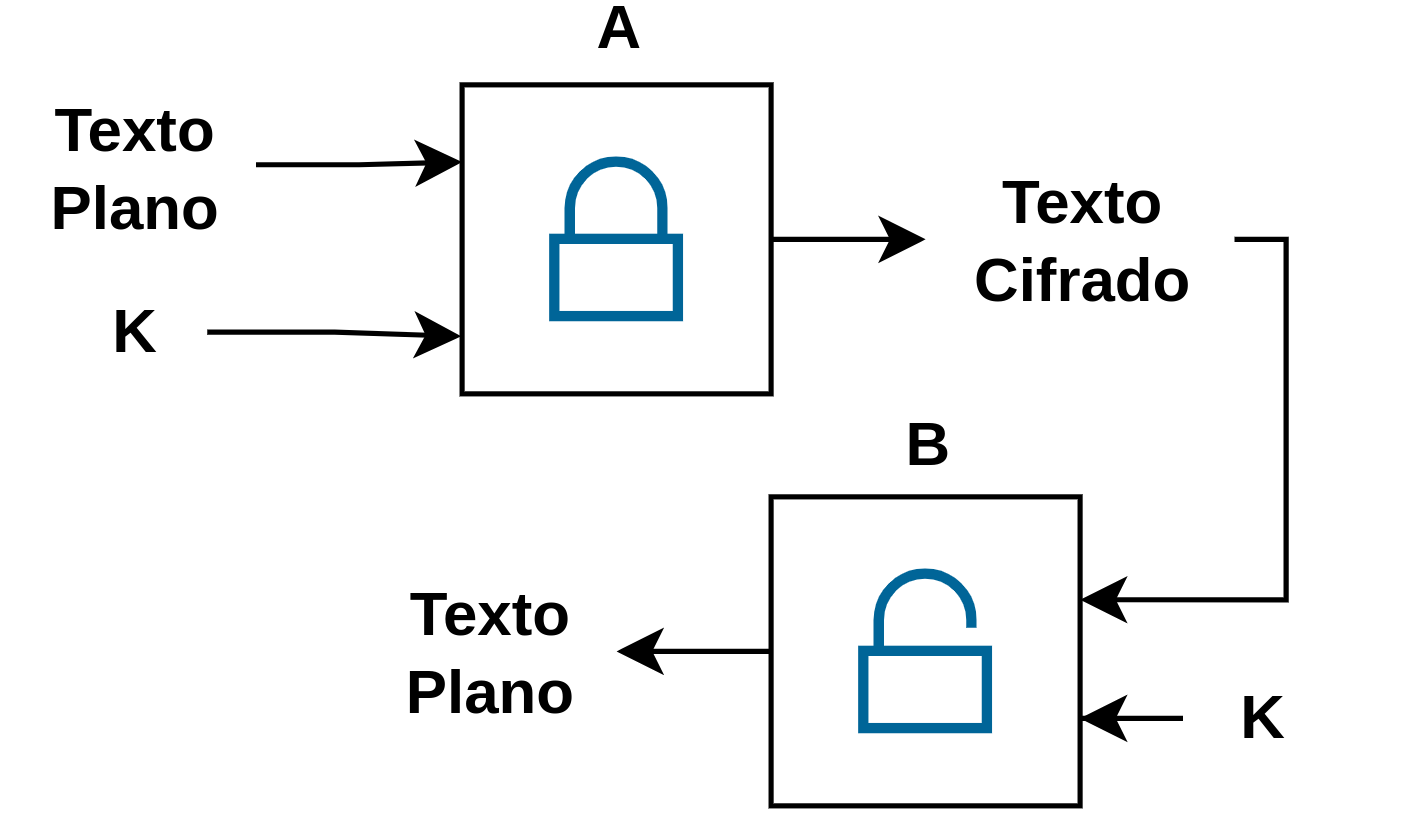
\includegraphics[width=\textwidth]{../figs/1_sim_encr.png}
        \caption{Encriptación simétrica}
        \label{fig:simetrica}
    \end{subfigure}
    \hfill
    \begin{subfigure}[b]{0.45\textwidth}
        \centering
        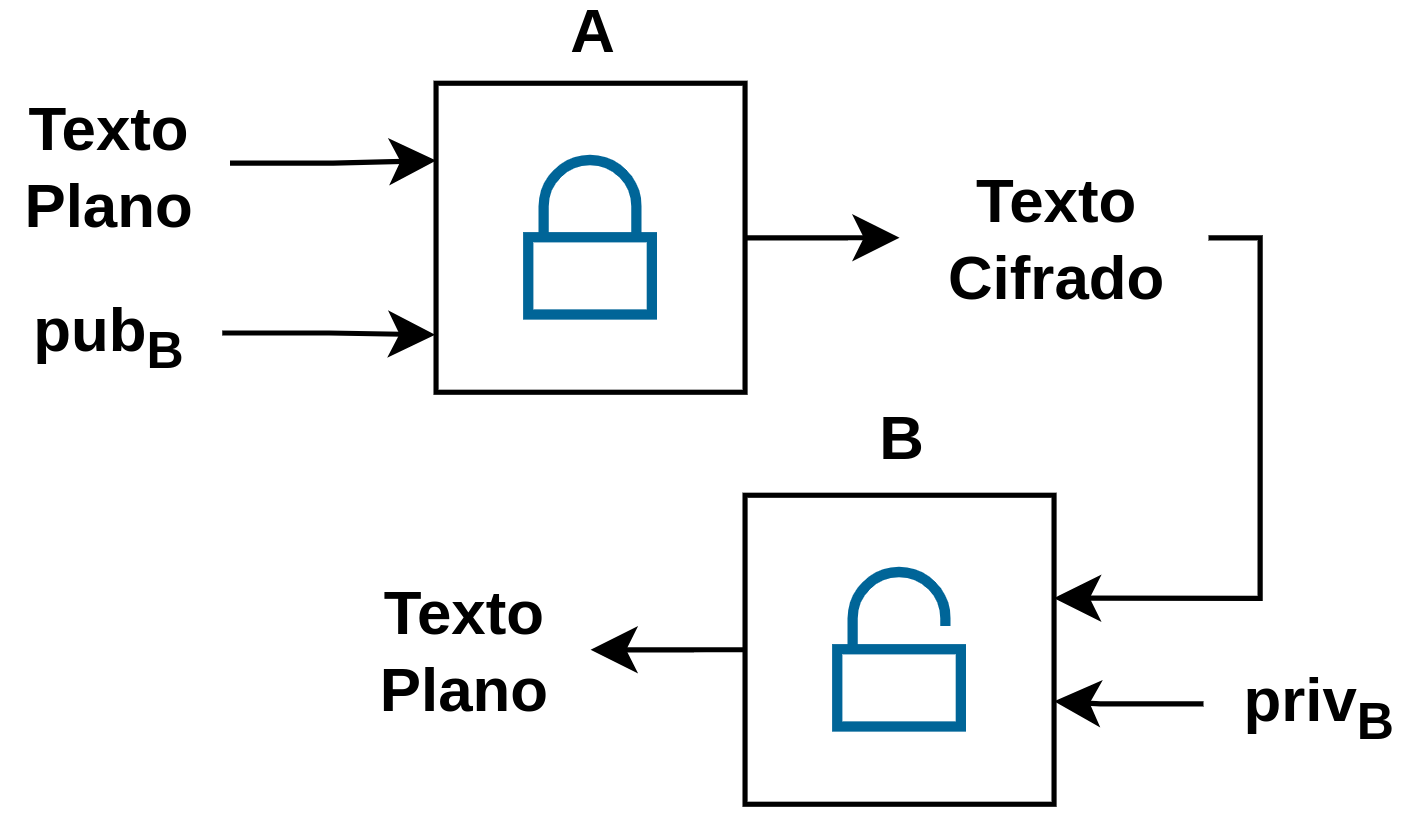
\includegraphics[width=\textwidth]{../figs/1_asim_encr.png}
        \caption{Encriptación asimétrica}
        \label{fig:asimetrica}
    \end{subfigure}
    \caption{Comparación entre encriptación simétrica y asimétrica.}
    \label{fig:encriptacion}
\end{figure}

%DIFFIE-HELLMAN
%CITAR PAPER ORIGINAL (REF EN WIKIPEDIA)
% REVISAR
\pdfcomment{REVISAR}
El método de Diffie-Hellmann propone combinar ambos enfoques para lograr acordar, empleando el concepto de encriptación asimétrica, una clave simétrica de manera segura que puede ser usada posteriormente para encriptar información. La principal ventaja del método radica en que ambas partes logran generar la misma clave simétrica sin transmitirla por el canal, mitigando un gran problema de seguridad del enfoque simétrico. La figura \ref{fig:diffie-hellmann} describe las operaciones matemáticas sobre las cuales funciona el método de Diffie-Hellmann.

\pdfcomment{
Acá voy a reemplazar la imagen por ecuaciones con las operaciones involucradas.}

\begin{figure}[h!]
    \centering
    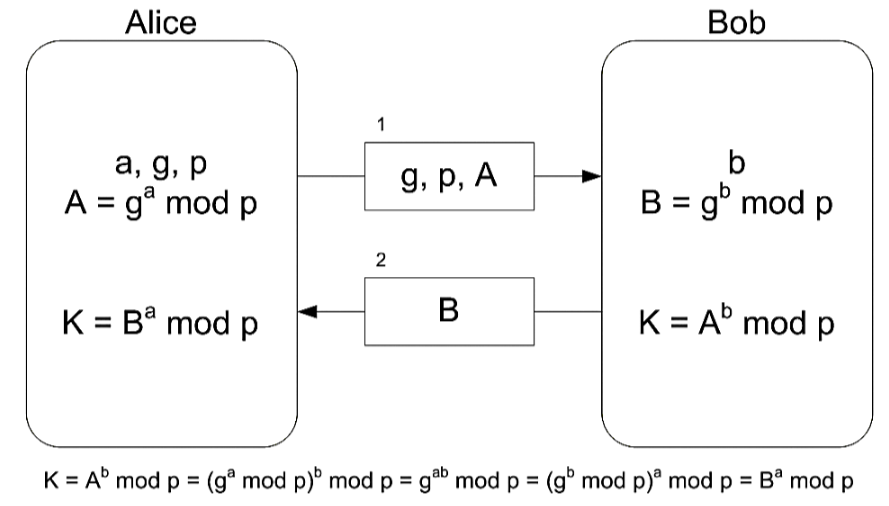
\includegraphics[width=0.4\textwidth]{../figs/1_diffie-hellmann.png}
    \caption{Método de Diffie-Hellmann para el acuerdo de una clave común.}
    \label{fig:diffie-hellmann}
\end{figure}

% MODIFICAR ESTO (LA CIA MODERNA UTILIZA COMBINACIONES DE DIFERENTES ALGORITMOS)
Para los estándares de seguridad actuales, un esquema de establecimiento de comunicaciones requiere mayor complejidad para abordar desafíos como un ataque de tipo man-in-the-middle. Aún así, el método de Diffie-Hellmann es la base de numerosas implementaciones por su simplicidad y el elevado costo computacional que supone calcular la clave K conociendo únicamente las claves públicas A y B.

\subsection{Suposiciones y restricciones}
Distintas soluciones de encriptación pueden proponerse según el nivel del modelo de capas que se analice. La encriptación a nivel de capa física minimiza las penalidades en rendimiento a costa de introducir complejidad al sistema, que se manifiesta en la necesidad de hardware dedicado de extremo a extremo de la red. Esta restricción puede volver inviable la encriptación a nivel de la capa física cuando el sistema de comunicaciones requiere de escalabilidad, principalmente por el costo de despliegue y mantenimiento.
La encriptación en capas superiores provee mayor flexibilidad en la implementación del sistema. Si bien esto introduce una mayor latencia a la red, reduciendo el rendimiento de la misma, se pueden lograr valores aceptables de latencia con suficiente optimización.  
Las soluciones de encriptación en la capa de red tienen la ventaja de ser independientes de la capa física, reduciendo la complejidad del sistema y permitiendo mayor flexibilidad en la implementación y compatibilidad con infraestructura preexistente. Esto implica que, cualquier sitio que cuente con una conexión a Internet y un dispositivo de encriptación tiene la infraestructura suficiente para acceder a una red segura, denominada red privada virtual.

En sistemas de criptografía, usualmente se utiliza el concepto de dominios rojo/negro para describir las partes del sistema que trabajan con información legible (dominio rojo) y aquellas que contienen información cifrada (dominio negro). La arquitectura de un sistema de comunicación seguro debe tener en cuenta este concepto para una correcta segregación de dominios, mitigando así la posibilidad de filtraciones indeseadas de información. La normativa actual que refiere a la segregación de dominios no contempla la segregación virtual, es decir, contener en un mismo dispositivo ambos dominios y aislarlos empleando herramientas de software. El implementar un sistema de este estilo capaz de cumplir las normas de seguridad existentes es un desafío importante.



\subsection{Resumen del sistema propuesto}

El sistema de comunicaciones seguras que se propone contempla el diseño de un único dispositivo, denominado encriptador, con la capacidad de formar un túnel VPN entre redes preexistentes, asegurando ciertos estándares de autenticación y confidencialidad sobre las comunicaciones entre dichas redes. El sistema opera a nivel de capa de red, y requiere de un mínimo de dos encriptadores para su funcionamiento, aunque también se encuentra prevista la escalabilidad del sistema.
El propósito del sistema es brindar confiabilidad respecto a la autenticación, confidencialidad e integridad de la información transmitida entre redes interconectadas,  afectando al mínimo el rendimiento de la red.

\begin{figure}[h!]
    \centering    
    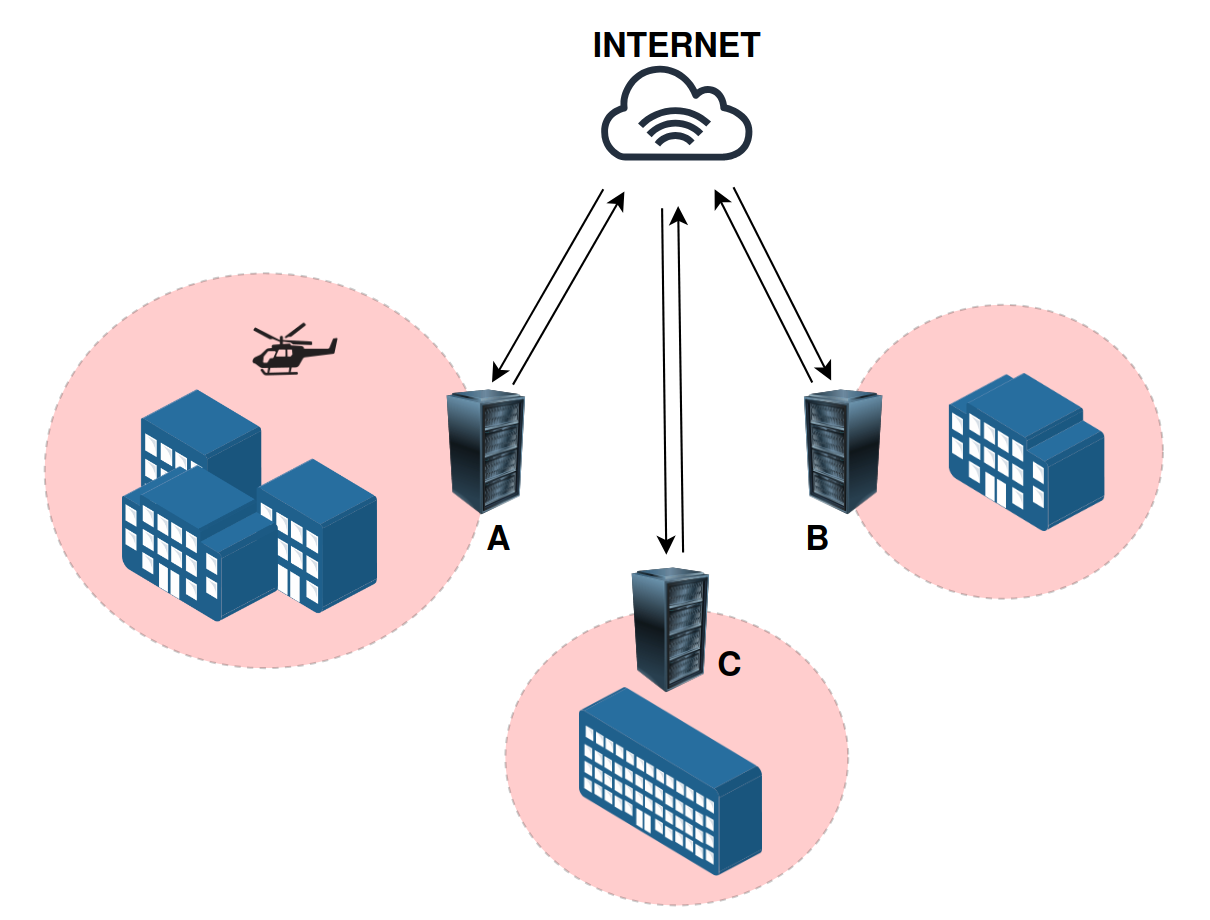
\includegraphics[width=0.4\textwidth]{../figs/1_overview.png}
    \caption{Esquema simplificado del sistema de comunicaciones seguras.}
    \label{fig:overview}
\end{figure}

En el esquema de la figura \ref{fig:overview} se describen los denominados dominios rojos, correspondientes a redes donde se trata con información sensible. El complemento de estos se denominan dominios negros, que usualmente se consideran canales inseguros donde la información proveniente de un dominio rojo requiere estar encriptada. 
El dispositivo encriptador actúa de interfaz entre dominios rojo y negro, motivo por el cual gran parte de la seguridad del sistema recae sobre este. Este dispositivo cuenta con acceso a claves utilizadas para establecer sesiones seguras con otros dispositivos, y al mismo tiempo cuenta con acceso a Internet. Debe poder garantizarse la seguridad en la gestión de estas claves y rechazar accesos no autorizados al dominio rojo.

\clearpage

\subsection{Objetivos, metas y justificación del sistema}

Un dispositivo en el cual los dominios rojo y negro no estén correctamente segmentados se encuentra con que la información confidencial respecto al túnel VPN como claves y permisos se hallan expuestos en el caso de una intrusión desde Internet o desde la propia red interna. Esto lleva a la posibilidad de que un agente no autorizado sea capaz de desencriptar y modificar información que viaje por el túnel, así como también acceder a dispositivos dentro de una organización.

En el diseño del encriptador, se propone implementar la segmentación virtual de dominios rojo/negro, esto es, representar los dominios como entidades virtuales independientes que ejecutan sobre hardware compartido. Este concepto puede implementarse a través de los denominados hipervisores, software que permite que varios sistemas operativos independientes trabajen juntos, compartiendo los mismos recursos físicos.

La segmentación permite que la entidad negra, la cual está conectada a Internet, realice el control del tráfico y oculte la existencia de la entidad roja para cualquier servicio fuera de la red virtual privada. Por otro lado, la entidad roja es la responsable de encriptar/desencriptar las comunicaciones entre organizaciones que se encuentren dentro de la red privada y de gestionar las claves de encriptación y los privilegios de usuarios. Esta segmentación permite un control estricto sobre el tráfico entre ambas entidades, mitigando la posibilidad de transferir información como claves contenidas en la entidad roja hacia la entidad negra.


\subsection{Usuarios y modos de operación}

\begin{center}
    \textbf{Usuarios}
\end{center}

\begin{itemize}
    \item \textbf{Administrador de red}: responsable de la configuración y mantenimiento del encriptador. Cuenta con acceso a la interfaz de administración del dispositivo y es el encargado de configurar el encriptador para funcionar dentro de la red segura. La configuración del encriptador incluye la definición de las redes que se conectarán a través del túnel VPN, la configuración de las claves de encriptación y la definición de los permisos de los usuarios.
    \item \textbf{Usuario final}: utiliza la red segura para compartir información sensible a otros nodos de la red. No tiene acceso a la configuración del encriptador y su interacción con el sistema se limita a utilizar la red segura como si de su red local se tratase.
\end{itemize}

\begin{center}
    \textbf{Modos de operación}
\end{center}

El diseño prevee que, una vez configurado el dispositivo, la operación del encriptador sea transparente para el usuario final, el cual no necesita interactuar con el dispositivo para utilizar la red segura.
\begin{itemize}
    \item \textbf{Nodo pequeño:} este modo de operación es de utilidad en sitios que no cuentan con infraestructura de red. El encriptador opera también como router, procesando todo el tráfico del sitio y permitiendo que el tráfico no destinado a otro sitio de la red segura sea enrutado por fuera del túnel VPN. Esta funcionalidad es conocida como \textit{split tunneling}. Es adecuado para instalaciones con tráfico moderado.
    \item \textbf{Nodo grande:} en instalaciones con tráfico elevado y que posiblemente cuenten con una infraestructura de red acorde, el equipo únicamente opera como encriptador de las comunicaciones seguras, y se conecta a un router preexistente para las comunicaciones no seguras. De esta manera solamente el tráfico dentro de la red segura es procesado por el encriptador.
\end{itemize}

\begin{figure}[h!]
    \begin{subfigure}{0.45\textwidth}
        \centering
        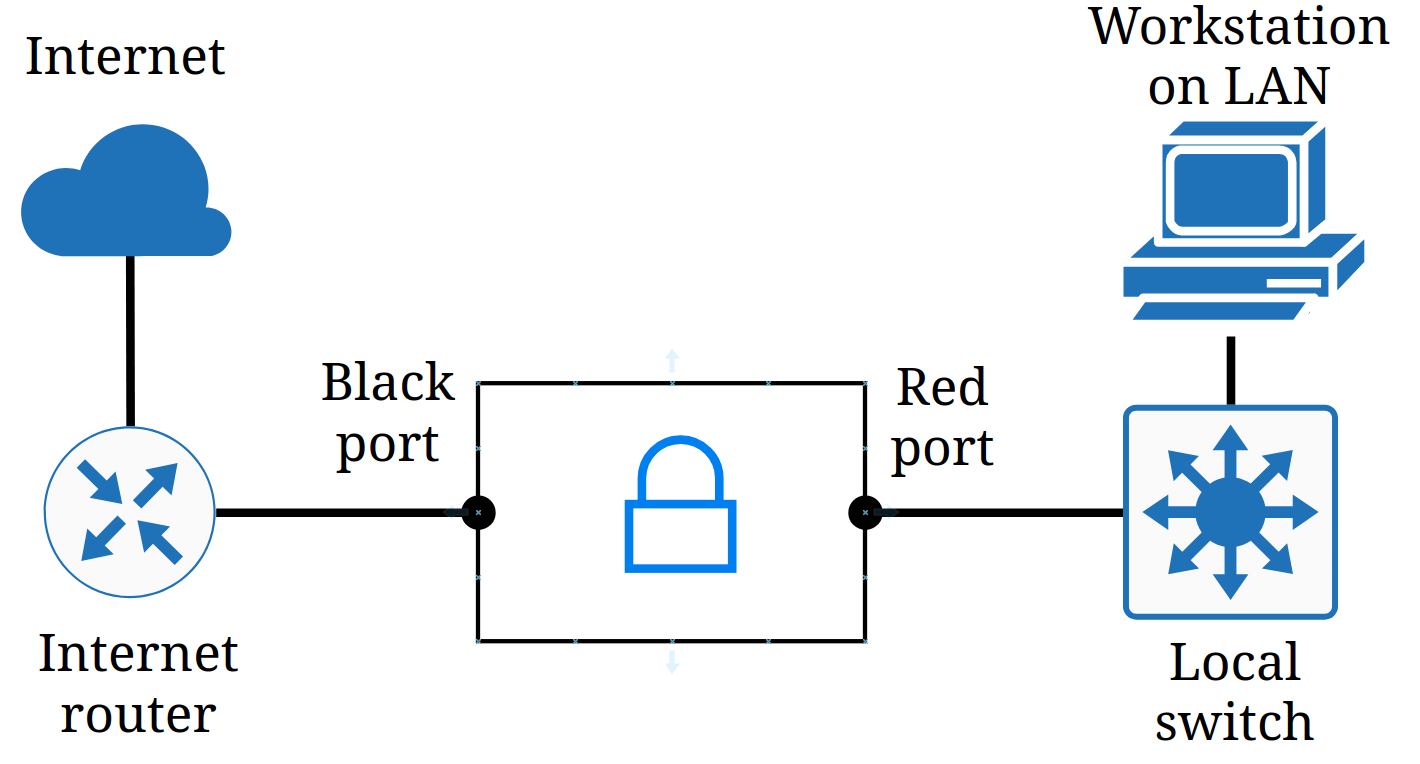
\includegraphics[width=\textwidth]{../figs/1_small_node.png}
        \caption{Sitio sin infraestructura de red.}
        \label{fig:small_node}
    \end{subfigure}
    \hfill
    \begin{subfigure}{0.45\textwidth}
        \centering
        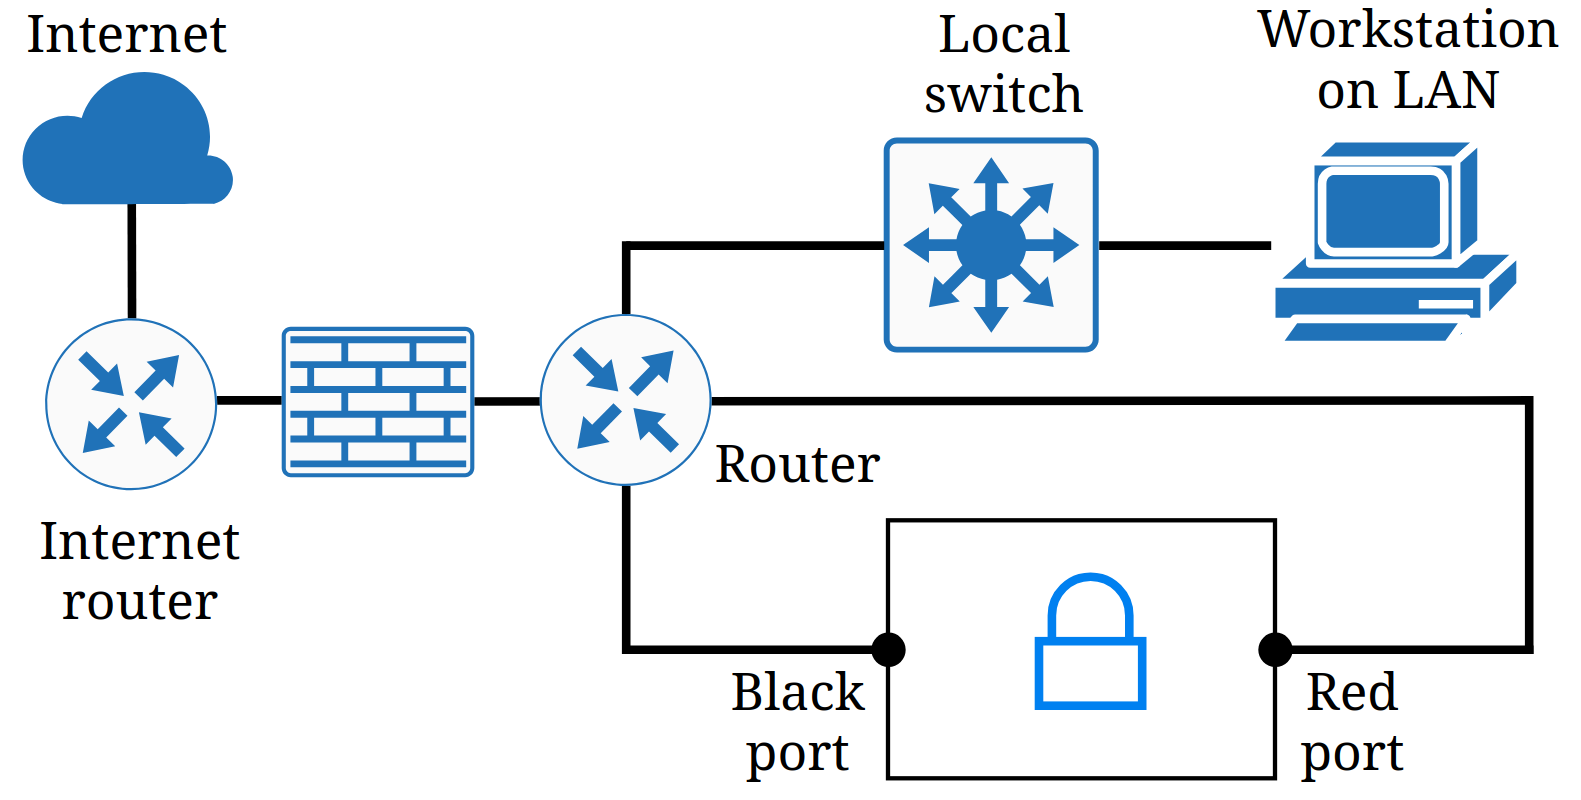
\includegraphics[width=\textwidth]{../figs/1_large_node.png}
        \caption{Sitio con infraestructura de red.}
        \label{fig:large_node}
    \end{subfigure}
    \caption{Modos de operación del encriptador.}
    \label{fig:modes_of_operation}
\end{figure}

\section{Requerimientos}
El documento de requerimientos es utilizado para describir que necesita el sistema para cumplir las necesidades de los usuarios. Esta sección establece las bases para la solución propuesta. Se definen a continuación las palabras clave que se utilizarán para referirse a los requerimientos:

\begin{table}[h!]
    \centering
    \begin{tabular}{|l|p{10cm}|}
        \hline
        \multicolumn{1}{|c|}{\textbf{Palabra clave}} & \multicolumn{1}{c|}{\textbf{Descripción}} \\
        \hline
        \textbf{DEBE} & Indica un requerimiento obligatorio que debe cumplirse para que el sistema funcione correctamente. \\
        \hline
        \textbf{NO DEBE} & Indica un requerimiento que no debe cumplirse, es decir, una restricción que debe evitarse. \\
        \hline
        \textbf{DEBERÍA} & Indica un requerimiento recomendado, pero no obligatorio. Se sugiere cumplirlo para mejorar la calidad del sistema. \\
        \hline
        \textbf{NO DEBERÍA} & Indica un requerimiento que se desaconseja cumplir, pero no es obligatorio evitarlo. \\
        \hline
        \textbf{PUEDE} & Indica una opción o característica que el sistema puede implementar, pero no es obligatoria. \\
        \hline
    \end{tabular}
    \caption{Palabras clave utilizadas en la definición de requerimientos.}
    \label{tab:palabras_clave_requerimientos}
\end{table}

\pdfcomment{
Adecuar todos los requerimientos según la tabla.}

\subsection{Funcionales}

\begin{itemize}
    \item \textbf{Renovación de claves:} cada par de nodos realiza una renovación de claves efímeras cada 120 segundos para asegurar forward-secrecy. Esto significa que, si una clave es comprometida por alguna razón, no se comprometen las comunicaciones anteriores o futuras fuera del intervalo de tiempo especificado.
    \item \textbf{Seguridad ante intrusiones:} el equipo debe ser capaz de  mitigar la posibilidad de intrusiones de agentes no autorizados vía software, tanto desde Internet o como desde la red local.
    \item \textbf{Detección de ataques DoS:} el sistema debe ser capaz de detectar y mitigar ataques de denegación de servicio.
    \item \textbf{Movilidad:} el sistema debe ser capaz de soportar la movilidad de los nodos y permitir a un nodo moverse entre redes sin interrupciones ni renegociaciones de claves. 
    \item \textbf{Split-tunneling:} el sistema debe ser capaz de permitir y enrutar tráfico de ciertas aplicaciones o servicios por fuera del túnel VPN. 
    \item \textbf{Segmentación de dominios: } el sistema debe aislar procesos contenidos en un dominio de información, como pueden ser archivos, contenida en otro dominio, independientemente de los privilegios que tenga este proceso.
\end{itemize}

\subsection{De rendimiento}

\begin{itemize}
    \item \textbf{Tasa de transferencia:} el sistema debe ser capaz de lograr, de un nodo a otro, una tasa de transferencia de 950 Mbits/s de datos planos.
    \item \textbf{Número de nodos:} una red segura debe ser capaz de soportar hasta 250 dispositivos encriptadores, también denominados nodos. 
\end{itemize}

\subsection{De interfaz}

\begin{itemize}
    \item \textbf{Administración:} la configuración de funcionamiento del  encriptador debe poder ser modificada únicamente por un administrador de red autorizado de manera local.
    \item \textbf{Interfaz de usuario:} el sistema debe ser transparente para el usuario final, es decir, no debe requerir de configuraciones adicionales para este.
    \item \textbf{Configuración de operación:} el modo de operación en red del sistema y otros parámetros de funcionamiento asociados deben ser configurables únicamente por el administrador de red.
\end{itemize}
\clearpage

\section{Descripción de tecnologías}
En este trabajo se combinarán distintas tecnologías que conformarán la solución final. A continuación se describen brevemente a modo de contextualizar al lector.

\subsection{WireGuard}
WireGuard es un protocolo de túneles VPN derivado de Noise Protocol Framework. Está diseñado para ser simple, rápido y eficiente, proporcionando una solución de código abierto con una base de código pequeña, lo que ayuda a minimizar la superficie de ataque. Su propósito es proporcionar una alternativa segura y eficiente a los protocolos VPN tradicionales, permitiendo la creación de túneles seguros entre dispositivos en una red. 

% Ejemplo de un archivo de configuración wg0.conf
\subsection{seL4}
Se trata de un microkernel con verificación formal matemática que garantiza que su implementación está libre de errores. Cuenta con una base de código muy reducida y proporciona un fuerte aislamiento entre procesos y una interfaz de comunicación segura. Es utilizado en sistemas críticos donde la seguridad y la confiabilidad son fundamentales. 

\subsection{CAmkES}
Trabajar con un microkernel como seL4 implica que la mayoría de las funcionalidades del sistema deben implementarse en el espacio de usuario. Para simplificar este proceso, seL4 incluye CAmkES, un \textit{framework} que facilita el desarrollo de sistemas de software modulares y seguros, diseñados específicamente para ejecutarse sobre seL4.

% \textcolor{blue}{Modular refiere a que CAmkES es un modelo de componentes. Seguro refiere a. Detallar el componente VMM, será utilizado después.}

% \begin{figure}[h!]
%     \centering
%     \includegraphics[width=0.5\textwidth]{example-image}
%     \caption{VMM.}
%     \label{diag:camkes_vmm}
% \end{figure}

% VirtQueue

% Comunicación VM - VMM - seL4 - Hardware




\chapter{Arquitectura propuesta}

\section{Arquitectura lógica}

\noindent\rule{\textwidth}{0.4pt}

Borrador:

\begin{itemize}
    \item Definir los criterios de diseño.
    \item Presentar la arquitectura lógica del sistema.
    \item Describir los componentes principales y sus interacciones.
    \item Incluir diagramas de componentes y de despliegue.
    \item Argumentar las decisiones de diseño tomadas.
\end{itemize}

\subsection{Dominios}

\noindent\rule{\textwidth}{0.4pt}



\section{Arquitectura física}

\noindent\rule{\textwidth}{0.4pt}
Borrador:

\begin{itemize}
    \item Describir las conexiones físicas entre los componentes del sistema.
    \item Passthrough.
\end{itemize}

\noindent\rule{\textwidth}{0.4pt}

\subsection{Hardware}

\clearpage

\chapter{Estrategia de modelos en entornos virtualizados}

Con el fin de abordar de manera ordenada la complejidad del sistema y validar progresivamente cada uno de sus componentes, se adoptó una estrategia basada en la construcción de modelos incrementales. Estos modelos permiten simular, probar y verificar distintas funcionalidades antes de integrarlas en la solución final.

Los modelos descritos a continuación tienen como finalidad:
\begin{itemize}
    \item Ligar problemas concretos a cada modelo y resolverlos de forma independiente. % Tener que debuggear todos en un solo modelo puede ser muy complejo.
    \item Obtener una solución funcional en un entorno virtualizado como último paso previo a implementarla sobre \textit{hardware}.
\end{itemize}

El detalle de cada modelo tiene como objetivo proporcionar una visión clara de su propósito, las validaciones que se intentan realizar y los aspectos que quedan fuera del alcance de cada uno. Además, en cada modelo se describen aspectos relevantes sobre las tecnologías utilizadas.

\section{Comunicando sitios seguros con WireGuard}
% Descripción del modelo
El primer modelo propuesto se centra en la comunicación entre múltiples sitios seguros a través de un túnel VPN configurado mediante WireGuard, permitiendo el acceso de los sitios a otros servicios en Internet por fuera del túnel. Se trata de un modelo de baja complejidad cuyo objetivo principal es familiarizarse con WireGuard y su configuración, así como utilizar herramientas como Wireshark para el análisis de paquetes de red. En una primera instancia, se implementó la topología de la figura \ref{diag:wg_minimal} utilizando GNS3, herramienta que permite instanciar y conectar múltiples máquinas virtuales, integrando herramientas de análisis de redes como Wireshark. 

Este modelo no pretende validar la arquitectura lógica del encriptador, sino que se enfoca en la configuración de WireGuard. Es por esto que cada encriptador se representa mediante una sola VM, en la cual se configura WireGuard. Se busca verificar que cada sitio pueda comunicarse con los demás a través del túnel VPN y acceder a Internet de manera directa.

Este modelo permite identificar y resolver problemas básicos de configuración de WireGuard, comprender el funcionamiento de las claves públicas y privadas, y analizar el tráfico cifrado y no cifrado mediante capturas en Wireshark.

\begin{figure}[h!]
    \centering
    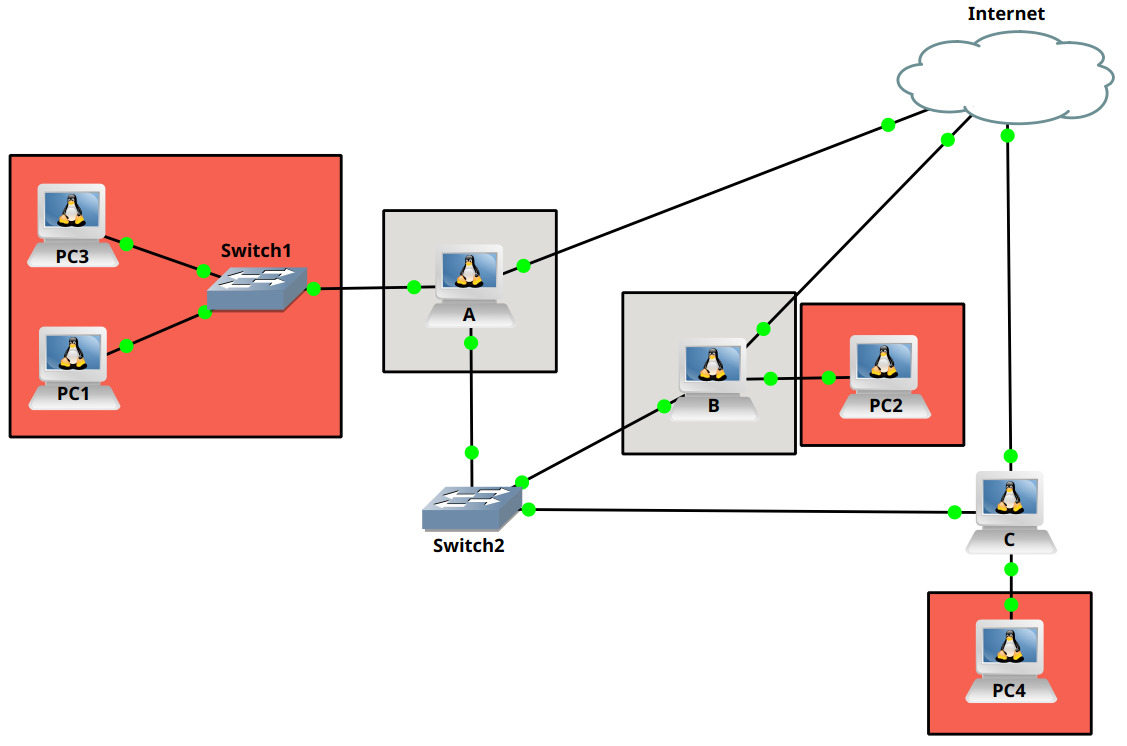
\includegraphics[width=0.6\textwidth]{../figs/gns3_1.png}
    \caption{Otro esquema mejorcito.}
    \label{diag:wg_minimal}
\end{figure}

En una siguiente iteración de este modelo se descartó la utilización de GNS3 y se optó por instanciar cada VM mediante QEMU% cosa que GNS3 ya lo hace en backend...
, adquiriendo mayor control sobre los dispositivos de red emulados. Un ejemplo de esto es la posibilidad de observar los parámetros PCI de las interfaces de red, lo cual es relevante para la implementación del \textit{passthrough} de las mismas en la solución final.

En este modelo, además, se valida el correcto funcionamiento tanto del kernel de Linux como del \textit{filesystem} inicial, modificados para incluir soporte para WireGuard. Estas imágenes serán posteriormente utilizadas en cada VMM gestionada por seL4.

\section{Introduciendo la arquitectura lógica del encriptador}
Una vez planteada la arquitectura lógica del sistema, se procedió con su simulación en GNS3. Este modelo permite limitar la complejidad de implementar la arquitectura a configurar la interconexión de las VMs que conforman el encriptador. Se tiene como objetivo validar la arquitectura lógica propuesta y verificar las funcionalidades de red pretendidas para el encriptador como lo es el \textit{split-tunneling}.

En la figura \ref{diag:gns3_2} se muestra la topología del modelo en GNS3 para simular el sistema completo. Aquí el encriptador se implementa como una interconexión mediante interfaces de red de tres VMs independientes. 

\begin{figure}[h!]
    \centering
    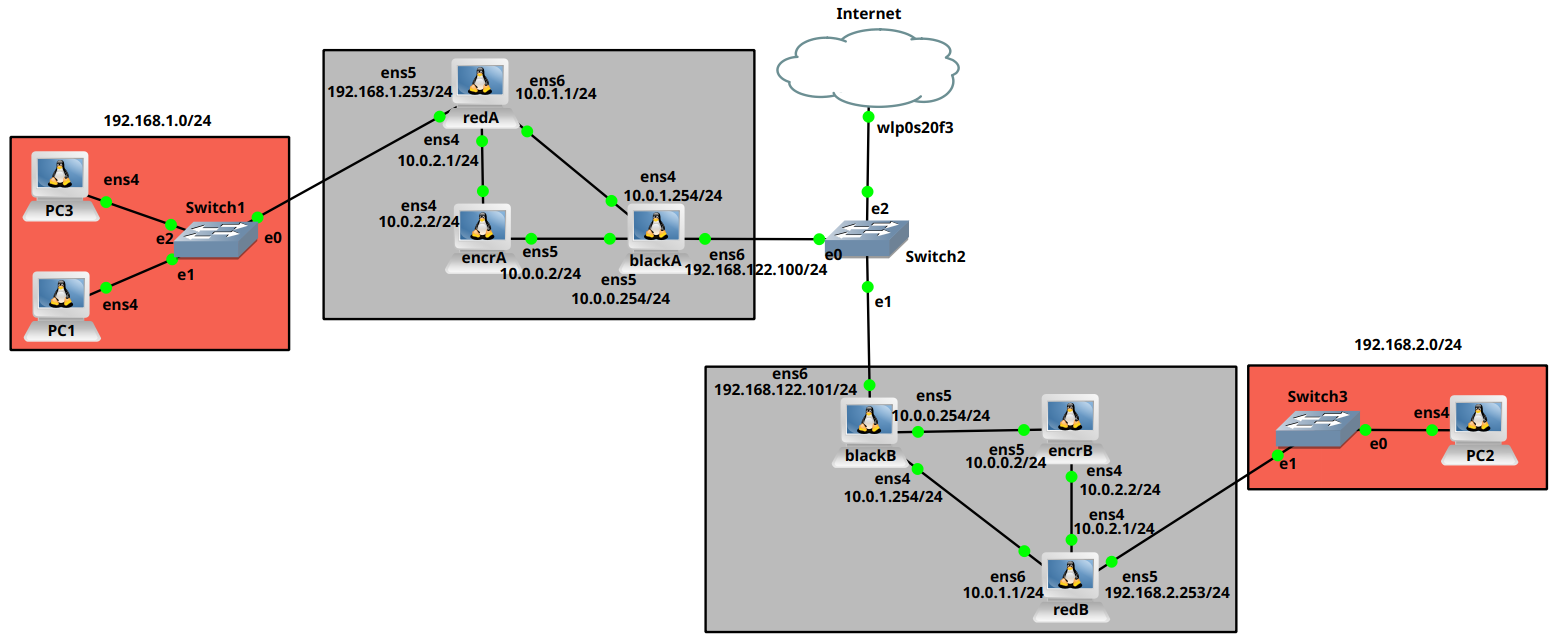
\includegraphics[width=0.8\textwidth]{../figs/gns3_2.png}
    \caption{Otro esquema mejorcito.}
    \label{diag:gns3_2}
\end{figure}

Como \textit{output} de este modelo se obtienen las configuraciones de red necesarias, como tablas de enrutamiento y reglas de firewall, para darle al encriptador la funcionalidad pretendida. Estas configuraciones se utilizarán posteriormente en la solución.

\section{Utilizando seL4 como hipervisor}
El siguiente modelo se centra en la lograr la comunicación entre dos VM, las cuales se encuentran en instancias independientes de seL4 funcionando como hipervisor. Este modelo tiene como objetivo validar el \textit{passthrough} de hardware, en este caso, de una interfaz de red entre seL4 y el \textit{guest} Linux. En la figura \ref{diag:esquema_passthrough} se esquematiza la topología del modelo.

\begin{figure}[h!]
    \centering
    \includegraphics[width=0.5\textwidth]{example-image}
    \caption{Dos VMs con un passthrough, ping 2VM.}
    \label{diag:esquema_passthrough}
\end{figure}

Un paso importante de este desarrollo es validar la compatibilidad de las imágenes de Linux obtenidas previamente con el hipervisor seL4. Para ello, en este modelo se utiliza el \textit{output} del primer modelo, la imagen de Linux con soporte para WireGuard.

Como \textit{output} de este modelo se tiene la configuración adecuada para realizar el \textit{passthrough} de un dispositivo de red al Linux \textit{guest}. Además de correcciones que se hayan hecho sobre la imagen de Linux para lograr la compatibilidad con el VMM de seL4.

\section{Implementando el encriptador en seL4}
Este modelo se centra en integrar los desarrollos realizados en los modelos anteriores, y obtener así una solución completa como paso previo a su despliegue sobre \textit{hardware} real. Aquí se validan en conjunto todas las funcionalidades y configuraciones obtenidas previamente, asegurando la interoperabilidad de los distintos componentes en un entorno virtualizado.

Este modelo utiliza uno de los ejemplos de uso de VMs en CAmkES, el proyecto \textit{zmq\_samples}, como base para la implementación del encriptador. Este ejemplo permite la comunicación entre dos VMs utilizando ZeroMQ, una biblioteca de mensajería asíncrona que facilita la comunicación entre procesos a través de regiones de memoria compartida definidas. Cada VM contiene una interfaz de red virtual \textit{eth0} que se conecta a las interfaces \textit{eth0} de las demás. En la figura \ref{diag:model4} se esquematiza el sistema completo.

\begin{figure}[h!]
    \centering
    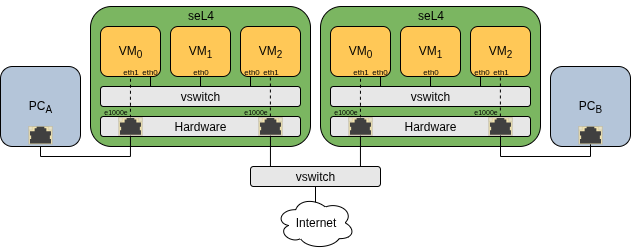
\includegraphics[width=0.8\textwidth]{../figs/3_model4.png}
    \caption{Esquema del encriptador con seL4 simulado en QEMU.}
    \label{diag:model4}
\end{figure}

\pdfcomment{
Describir el cambio de topología respecto a la figura \ref{diag:gns3_2}. ¿Por qué esto no afecta?}



\chapter{Implementación en entorno virtualizado} % sistema completo seL4 en QEMU
\section{Diseño del experimento}
\begin{itemize}
    \item Se realizará en completamente en host. ¿Por qué? Simplicidad de implementación.
\end{itemize}
\section{Procedimiento} % Proceso de: linux_QEMU-linux_QEMU -> 3VMsel4_QEMU. 3VMsel4_QEMU
\pdfcomment{
Describir que necesita seL4 para funcionar como queremos}

\subsection{Generación de una imagen de sistema mediante Buildroot}
Buildroot es una herramienta que permite generar imágenes de sistema de archivos o \textit{root filesystem} minimalistas para sistemas embebidos. Es útil para crear sistemas operativos ligeros y personalizados, adaptados a las necesidades específicas de un proyecto. Se utilizó Buildroot para generar una imagen de sistema que contenga los binarios necesarios para el funcionamiento de WireGuard y otras herramientas de red requeridas.
En este trabajo se provee el archivo de configuración utilizado para la versión 2023.02.1 de Buildroot y se detalla a continuación el procedimiento para replicar la imagen.
\pdfcomment{
Citar o referenciar el repositorio PI-2025-IB de alguna forma}

\begin{lstlisting}[caption={Generación de imagen de sistema con Buildroot.}, label={lst:buildroot_procedure}]
git clone --branch 2023.11 https://github.com/buildroot/buildroot.git
cp .buildroot-config ./buildroot/.config
cd buildroot
make
\end{lstlisting}

\subsection{Construcción de un kernel Linux con soporte para WireGuard}
Actualmente, el VMM de seL4 implementado en CAmkES para la arquitectura x86 cuenta con soporte probado para el kernel Linux 4.9. En este trabajo se utilizó una versión limpia de este kernel, obtenida de la rama \textit{stable} de Linux 4.9.y, en particular la versión 4.9.337, que se encuentra disponible en el repositorio oficial de Linux. Al momento de configurar la compilación del kernel, se tuvo en cuenta la compatibilidad con el hipervisor seL4, cuyos requisitos se encuentran documentados en la página oficial del proyecto \textit{camkes-vm} para seL4 \cite{camkes_vm}.
\pdfcomment{
Agregar codigo para compilar el kernel}

El soporte nativo para WireGuard fue añadido al kernel Linux en la versión 5.6, sin embargo, el repositorio \textit{wireguard-linux-compat} provee un parche que permite compilar WireGuard en versiones anteriores del kernel, como la utilizada \cite{wireguard-compilation}.

\begin{lstlisting}[language=bash, caption={Parche wireguard-linux-compat para el kernel Linux 4.9.337}, label={lst:wireguard_patch}]
git clone https://git.zx2c4.com/wireguard-linux-compat
./wireguard-linux-compat/kernel-tree-scripts/jury-rig.sh ./linux-stable
\end{lstlisting}


\subsection{Adaptación del proyecto \textit{zmq\_samples}}
\subsubsection{Utilización de kernel modificado}
En la configuración por defecto de este proyecto se cuenta con las imágenes de sistema para un kernel Linux 4.8.16 en cada VM. Para utilizar las imágenes de sistema generadas en pasos anteriores se realizaron modificaciones en el archivo \textit{CMakeLists.txt} del proyecto, ubicado en el directorio \textit{camkes-vm-examples-manifest/projects/vm-examples/apps/x86/zmq\_samples/}. En este archivo se definieron las rutas de los archivos a utilizar mediante las siguientes variables CMake:

\begin{lstlisting}[caption={Variables CMakeLists.txt del proyecto zmq\_samples}, label={lst:zmq_samples_cmake}]
set(kernel_file "/host/custom-vm-kernel/linux-stable/arch/x86/boot/bzImage")
set(rootfs_file "/host/custom-vm-kernel/buildroot/output/images/rootfs.cpio")
\end{lstlisting}

\subsubsection{Gestión de memoria de las VMs}
En seL4, toda la memoria física se inicia como \textit{untyped memory}, lo que significa que no está asignada a ningún objeto específico. A medida que se crean objetos, como VMMs, se realizan asignaciones de memoria, convirtiendo parte de la memoria \textit{untyped} en memoria \textit{typed}. Una característica importante de la gestión de memoria en seL4 es que la alocación es estática para objetos en kernel. Esto implica que, al crear una VM, se debe definir la cantidad de memoria que se le asignará desde el inicio. Esta cantidad no puede ser modificada posteriormente, lo que requiere una planificación cuidadosa para evitar problemas de memoria insuficiente durante la ejecución de las VMs. \pdfcomment{Acá puedo citar al manual de seL4 sección 2.4}

Cuando se hace uso del VMM \textit{camkes-vm} se tienen los siguientes parámetros de configuración directamente relacionados al uso de memoria de un \textit{guest}:
\begin{itemize}
    \item \texttt{simple\_untypedN\_pool}: CAmkES realiza una prealocación de memoria \textit{untyped} para ser gestionada por cada VM. Aquí \texttt{N} representa una máscara sobre la cantidad de bits que definen el tamaño del bloque de memoria. Por ejemplo, \texttt{vm0.simple\_untyped23\_pool = 10} indica que se reservan 10 bloques de memoria de 2\textsuperscript{23} bytes (8 MB) para el componente \texttt{vm0}. Una forma de dar flexibilidad al sistema es definir \textit{pools} de memoria \textit{untyped} de diferentes tamaños. 
    \item \texttt{heap\_size}: este parámetro define el tamaño del \textit{heap} del componente VMM. Es memoria reservada para el uso del VMM si este requiere por ejemplo guardar información de estado o utilizar buffers de datos. La asignación \texttt{vm0.heap\_size = 0x40000} define 256 KiB de memoria para el \textit{heap} del componente VMM correspondiente a \texttt{vm0}.
    \item \texttt{guest\_ram\_mb}: la memoria RAM disponible para la VM es simplemente la asignación de memoria \textit{untyped} disponible en \textit{pools} reservados para la misma. Por ejemplo, \texttt{vm0.guest\_ram\_mb = 128} indica que se asignarán 128 MB de memoria RAM a la VM \texttt{vm0}. Es importante tener en cuenta que este valor no puede superar a la cantidad de memoria \textit{untyped} reservada para la VM.
\end{itemize}
Por defecto se definen\dots


\subsubsection{Configuración del \textit{passthrough} de interfaz Ethernet}
\begin{itemize}
    \item Interfaz e1000 QEMU. PCI. BARS. IRQ.
    \item Modificar la configuración de la VMM camkes en seL4 para permitir el acceso a los recursos PCI correspondientes.
    \item Solución al problema de utilizar dos interfaces de red. Diferentes IRQ.
    \item Funcionamiento de passthrough (colas).
\end{itemize}

\section{Integración}
\begin{itemize}
    \item Bridge en host. 4 instancias de QEMU. 2 PCs y 2 encriptadores.
\end{itemize}

\section{Validación} %verificar requerimientos


\chapter{Implementación en hardware}
    \section{SuperMicro SYS-E300-9D}
    \begin{itemize}
        \item Supermicro server sys-e300-9d with X11SDV-4C-TLN2F motherboard and intel xeon D-2123IT. Fotito del equipo.
        \item IPMI, COM1, SoL.
    \end{itemize}
    \section{Diseño del experimento}
    \begin{itemize}
        \item Que cosas esperamos validar. Rendimiento y que más?
        \item SetUP.
    \end{itemize}
    \section{Procedimiento}
    \begin{itemize}
        \item 1. Configurar redirección consola serie.
        \item 2. Bootear el Linux para obtener los parámetros para configurar el zmq\_samples (lspci).
        \item 
    \end{itemize}

\chapter{Implementación en entorno virtualizado} % sistema completo seL4 en QEMU
\section{Diseño del experimento}
\begin{itemize}
    \item Se realizará en completamente en host. ¿Por qué? Simplicidad de implementación.
\end{itemize}
\section{Procedimiento} % Proceso de: linux_QEMU-linux_QEMU -> 3VMsel4_QEMU. 3VMsel4_QEMU
  
\subsection{Construcción de un kernel Linux con soporte para WireGuard}
\begin{itemize}
    \item De www.wireguard.com/compilation/kernel-requirements se obtuvieron los requerimientos.
    \item wireguard-linux-compat patch
    \item seL4 soporta kernel 4.9[ref], se compiló este kernel con una adaptación de .config file original de los ejemplos camkes-vm
    \item Buscar referencias para justificar todo. \cite{Laricch2009AAMOP_ICBp3}

    \item Drivers de red compatibles con el hardware utilizado.
\end{itemize}

\subsection{Generación de una imagen de sistema mediante Buildroot}
\begin{itemize}
    \item Se utilizó la versión 2023.02.1 de Buildroot utilizando el kernel modificado.
    \item Se configuró el sistema de archivos para que contenga los binarios necesarios para el funcionamiento de WireGuard y las herramientas de red.
\end{itemize}

\subsection{Adaptación del ejemplo \textit{zmq\_samples}}
\begin{itemize}
    \item Se adaptó el ejemplo de CAmkES para que funcione con el nuevo kernel y la imagen de sistema generada. Basicamente tocar el CMakeLists.txt
    \item ZeroMQ. Problema con iperf3 solucionado aumentando tamaño de buffers.
    \item Incrementar RAM de las VMs.
\end{itemize}

\subsection{Configuración del \textit{passthrough} de interfaz Ethernet}
\begin{itemize}
    \item Interfaz e1000 QEMU. PCI. BARS. IRQ.
    \item Modificar la configuración de la VMM camkes en seL4 para permitir el acceso a los recursos PCI correspondientes.
    \item Solución al problema de utilizar dos interfaces de red. Diferentes IRQ.
    \item Funcionamiento de passthrough (colas).
\end{itemize}

\section{Integración}
\begin{itemize}
    \item Bridge en host. 4 instancias de QEMU. 2 PCs y 2 encriptadores.
\end{itemize}

\section{Validación} %verificar requerimientos

\chapter{Implementación en hardware}
    \section{SuperMicro SYS-E300-9D}
    \begin{itemize}
        \item Supermicro server sys-e300-9d with X11SDV-4C-TLN2F motherboard and intel xeon D-2123IT. Fotito del equipo.
        \item IPMI, COM1, SoL.
    \end{itemize}
    \section{Diseño del experimento}
    \begin{itemize}
        \item Que cosas esperamos validar. Rendimiento y que más?
        \item SetUP.
    \end{itemize}
    \section{Procedimiento}
    \begin{itemize}
        \item 1. Configurar redirección consola serie.
        \item 2. Bootear el Linux para obtener los parámetros para configurar el zmq\_samples (lspci).
        \item 
    \end{itemize}



\appendix
\chapter{Apéndice I}\label{C:ap1}
%\chapterquote{Negociemos Don Inodoro}{Fernando de la R\'{u}a, 2001}
\graphicspath{{figs/}}
%%%%%%%%%%%%%%%%%%%%%%%%%%%%%%%%%%%%%%%%%%%%%%%%%%%%%%%%%%%%%%%%%%%%%%%%



%%% Local Variables: 
%%% mode: latex
%%% TeX-master: "template"
%%% End: 


\begin{biblio}
\bibliography{mibib}
\end{biblio}


\begin{postliminary}

\begin{seccion}{Publicaciones asociadas}
  \begin{enumerate}
  \item Mi primer aviso en la revista \textbf{ABC}, 1996
  \item Mi segunda publicaci\'{o}n en la revista \textbf{ABC}, 1997
  \end{enumerate}
\end{seccion}

\begin{seccion}{Agradecimientos}
A todos los que se lo merecen, por merecerlo
\end{seccion}

\end{postliminary}

\end{document}

